\documentclass[conference]{IEEEtran}
\IEEEoverridecommandlockouts
% The preceding line is only needed to identify funding in the first footnote. If that is unneeded, please comment it out.

\usepackage[acronym]{glossaries}
\usepackage{cite}
\usepackage{amsmath,amssymb,amsfonts}
\usepackage{algorithmic}
\usepackage{graphicx}
\usepackage{textcomp}
\usepackage{xcolor}

\usepackage{listings}
% \usepackage{biblatex}
\usepackage{adjustbox}
\usepackage{tabulary}

\usepackage{todonotes}
\newcommand{\db}[1]{\textcolor{blue!40}{#1}}
\newcommand{\dbc}[1]{\todo[author=Dilum, inline, color=blue!40]{#1}}
\newcommand{\gk}[1]{\textcolor{orange}{#1}}
\newcommand{\gkc}[1]{\todo[author=Gihan, inline, color=green!40]{#1}}

\usepackage{hyperref}
\usepackage{cleveref}

\crefformat{section}{#2Sec.~#1#3}
\crefformat{figure}{#2Fig.~#1#3}
\crefformat{table}{#2Table~#1#3}

% \addbibresource{mendeley.bib}

\definecolor{codegreen}{rgb}{0,0.6,0}
\definecolor{backcolour}{rgb}{0.95,0.95,0.92}
\lstdefinestyle{code-style}{
  backgroundcolor=\color{backcolour}, commentstyle=\color{codegreen},
  basicstyle=\ttfamily\footnotesize,
  breakatwhitespace=false,
  breaklines=true,
  captionpos=b,
  keepspaces=true,
  numbers=left,
  numbersep=1pt,
  showspaces=false,
  showstringspaces=false,
  showtabs=false,
  tabsize=1
}
\lstset{style=code-style}

\def\BibTeX{{\rm B\kern-.05em{\sc i\kern-.025em b}\kern-.08em
    T\kern-.1667em\lower.7ex\hbox{E}\kern-.125emX}}
    
\begin{document}

\title{WDIAS: A Microservices-Based Weather Data Integration and Assimilation System\\
}

\author{\IEEEauthorblockN{Gihan Karunarathne}
\IEEEauthorblockA{\textit{Dept. Computer Science and Engineering} \\
\textit{University of Moratuwa}\\
Katubedda, Sri Lanka \\
gihan.09@cse.mrt.ac.lk}
\and
\IEEEauthorblockN{H.M.N. Dilum Bandara}
\IEEEauthorblockA{\textit{Dept. Computer Science and Engineering} \\
\textit{University of Moratuwa}\\
Katubedda, Sri Lanka \\
dilumb@cse.mrt.ac.lk}
\and
\IEEEauthorblockN{Srikantha Herath}
\IEEEauthorblockA{\textit{Center for Urban Water, Sri Lanka} \\
Battaramulla, Sri Lanka \\
admin@curwsl.org}
}

\maketitle

%%%%%%%%%%%%%%%%%%%%%%%%%%%%%%%%%%%%%%%%%%%%%%%%%%%%%%%%%%%%%%%%%%%%%%%%%%%%%%%%
\begin{abstract}
Numerical Weather Models (NWMs) utilize data from diverse sources such as automated weather stations, radars, and satellite images. Such multimodal data need to be transcoded into a NWM compatible format before use. Moreover, the data integration system's response time needs to be relatively low to reduce the time to forecast weather events like hurricanes and flash floods. Furthermore, the resulting data need to be accessed by many researchers and third-party applications. Existing weather data integration systems are based on monolithic or client-server architectures, and are proprietary or closed source. Hence, they are not only expensive to operate in an era of cloud computing, but also challenging to customize for regions with different weather patterns. In this paper, we present a Weather Data Integration and Assimilation System (WDIAS) that uses microservices architecture and container orchestration to achieve high scalability, availability, and low-cost operation. WDIAS provides a modular architecture to integrate data from different sources, enforce data quality controls, export data into different formats, and extend the functionality by adding new modules. Using a synthetic workload and an experimental setup on a public cloud, we demonstrate that WDIAS can handle 300 requests per second with relatively low latency.
\end{abstract}


\begin{IEEEkeywords}
Cloud computing, data assimilation, data integration, microservice, weather
\end{IEEEkeywords}

%%%%%%%%%%%%%%%%%%%%%%%%%%%%%%%%%%%%%%%%%%%%%%%%%%%%%%%%%%%%%%%%%%%%%%%%%%%%%%%%
\section{Introduction}
\label{pse:Introduction}

Weather prediction is essential to reduce impact due to natural disasters and to manage natural resources like water effectively. To enhance the accuracy of weather predictions, it is necessary to provide reliable and detailed weather data as inputs to \acrfull{nwm}s. Before feeding multimodal data collected from different sources into a NWM, they need to be converted to a format that can be ingested by the NWM. Further, the velocity and volume of data vary from event-driven bulk uploads to streaming data. Such data need to be ingested, converted, stored, and accessed with minimal latency, especially when forecasting time-sensitive weather events. Processed weather data may also need to be accessed by many third-party applications and researchers. For example, logistics and insurance companies could use weather data for planning purposes or set their service fees or premiums based on anticipated weather patterns.

Several data integration systems are designed for weather-related use cases. For example, \acrshort{fews} \cite{Werner2013TheSystem} uses a model-centric approach where it handles the forecasting process as a combination of data modeling steps and data transformation algorithms. It creates forecasting workflows by integrating new models and algorithms based on the open model integration framework \cite{Kokkonen2003InterfacingXML}. \acrshort{fews} follows a common data model and enforces data access via a well-defined interface. While such a design leads to efficient data access and management, it requires all NWMs and connected systems to comply with the common data model, tightly couples the models, and serializes the model execution. 
\acrfull{lead} \cite{Droegemeier2005Service-OrientedWeather} provides dynamic workflow orchestration and data management based on Web-services. It provides several service layers based on the \acrfull{soa}, exposes services via a drag-and-drop interface to create new workflows, and aggregates computing resources into a pool. This design design results in a high performing, customizable, scalable, and resource-efficient weather analysis framework. 
\acrfull{dias} \cite{Kawasaki2018DataReduction} is another related system that provides efficient data storage, data quality controls, metadata management, and data sharing. \acrfull{madis} \cite{Macdermaid2005ArchitectureP2.39} enforces a common data format and provides role-based data access. 
However, \acrshort{dias} and \acrshort{madis} do not support workflows. All these systems are based on monolithic or client-service architectures and are platform dependent. Thus, they cannot gain the performance and economic benefits of contemporary technologies such as cloud computing. Further, these systems are either proprietary or closed source, limiting the wider adoption and customization. For example, it is challenging to customize them for an island like Sri Lanka with different weather patterns.

In this paper, we present a cloud-based \acrfull{wdias} that supports data integration, assimilation, and dissemination. We designed the proposed system based on the microservices architecture to make it highly scalable, available, modular, and extensible compared to related systems. \acrshort{wdias} can integrate both bulk and timeseries data from different sources, export data into different formats, and add extension modules for custom data transformations and quality controls. The proposed platform further uses container orchestration to simplify application management and gain cost savings through efficient use of cloud computing resources. 
Using an experimental setup on the cloud and synthetic workload derived from weather use cases, we demonstrate that \acrshort{wdias} can handle 300 requests (with different data types) per second. Also, the system is capable of running on a large range of computing resources ranging from a few CPUs to hundreds of CPUs, as well as show good elasticity against varying workloads.

The rest of the paper is organized as follows: The architecture of \acrshort{wdias} is presented in \cref{pse:wdias_architecture}. In \cref{pse:performance_analysis} we present the performance analysis. Concluding remarks are presented in \cref{pse:summary}.

%%%%%%%%%%%%%%%%%%%%%%%%%%%%%%%%%%%%%%%%%%%%%%%%%%%%%%%%%%%%%%%%%%%%%%%%%%%%%%%%

\begin{figure}[!tb]
\centerline{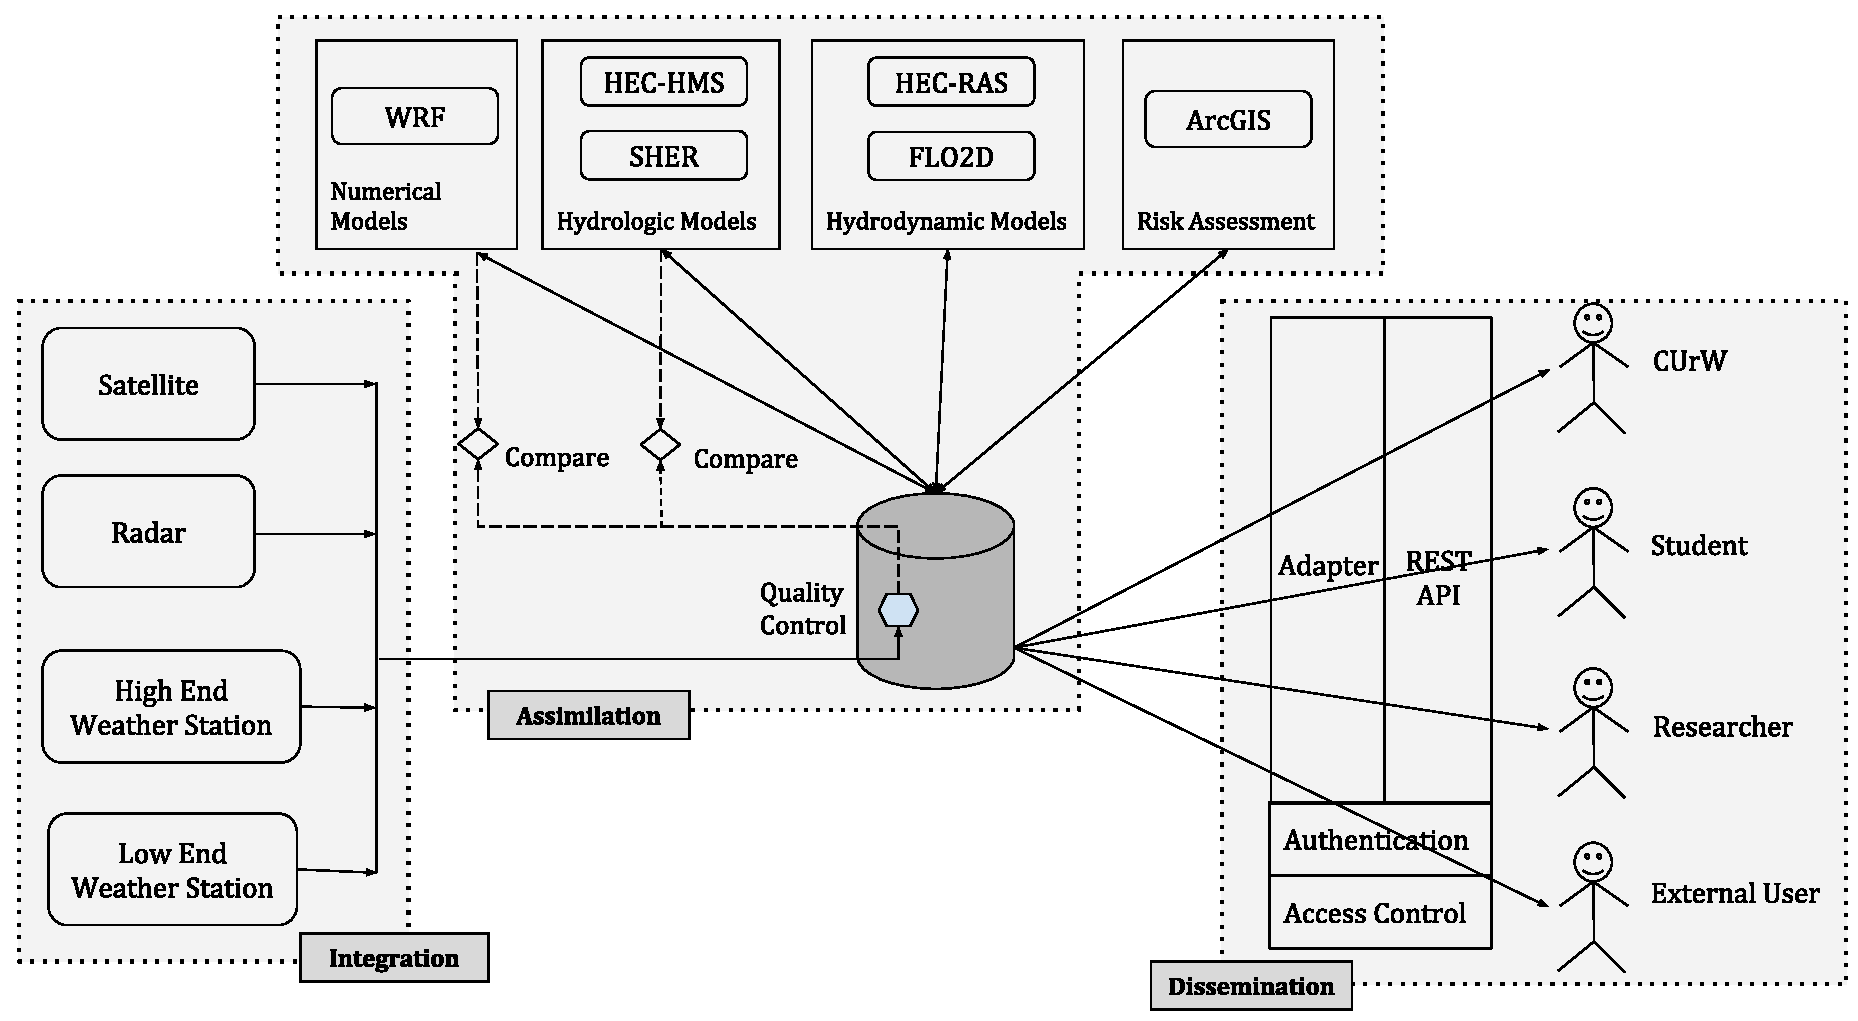
\includegraphics[width=0.5\textwidth]{images/weather_data_system_components_p1.pdf}}
\caption{Components of a weather data integration and assimilation system.}
\label{pfi:wdia_components}
\end{figure}

%%%%%%%%%%%%%%%%%%%%%%%%%%%%%%%%%%%%%%%%%%%%%%%%%%%%%%%%%%%%%%%%%%%%%%%%%%%%%%%%
\section{Proposed Architecture}
\label{pse:wdias_architecture}

%%%%%%%%%%%%%%%%%%%%%%%%%%%%%%%%%%%%%%%%%%%%%%%%
\subsection{WDIAS Microservices Architecture}
\label{psubse:wdias_microservices}

\cref{pfi:wdia_components} shows the essential functions of a weather data integration and assimilation system such as integration, assimilation, and dissemination. A typical system should be capable of integrating multimodal and multidimensional spatial and temporal weather data from diverse sources such as satellites, radars, and high-end and low-end weather stations. In assimilation, the system not only stores the data but also provides them to various weather models in their desired data formats. In the dissemination step, both the captured weather data and processed data from weather models are shared with users and external systems based on their data subscriptions, timeseries metadata and geo-tag based queries, and access rights. \acrshort{wdias} supports all three of these modules.

We used microservices architecture for \acrshort{wdias}, as it enables resilient and flexible services that can be independently scaled while achieving high-availability \cite{LewisMicroservices}. Such a design allows each module to be offered as a separate microservice where each module works on a separate piece of bulk or stream data. Microservices further enables modules to be written in any language and dynamically added to the system to extend its functionality. We implemented services as containerized applications, which further simplifies the deployment and maintenance of services on a cloud platform resulting in simplified administration and cost savings. Application containerization is an alternative to virtualization where a software and all its dependencies are encapsulated/grouped into a container that can execute uniformly and consistently in any infrastructure \cite{IBMContainerizationExplained}. Containerization has emerged as an industry standard for packaging software into standardized units for development, shipment, and deployment.


\begin{figure}[!tb]
\centerline{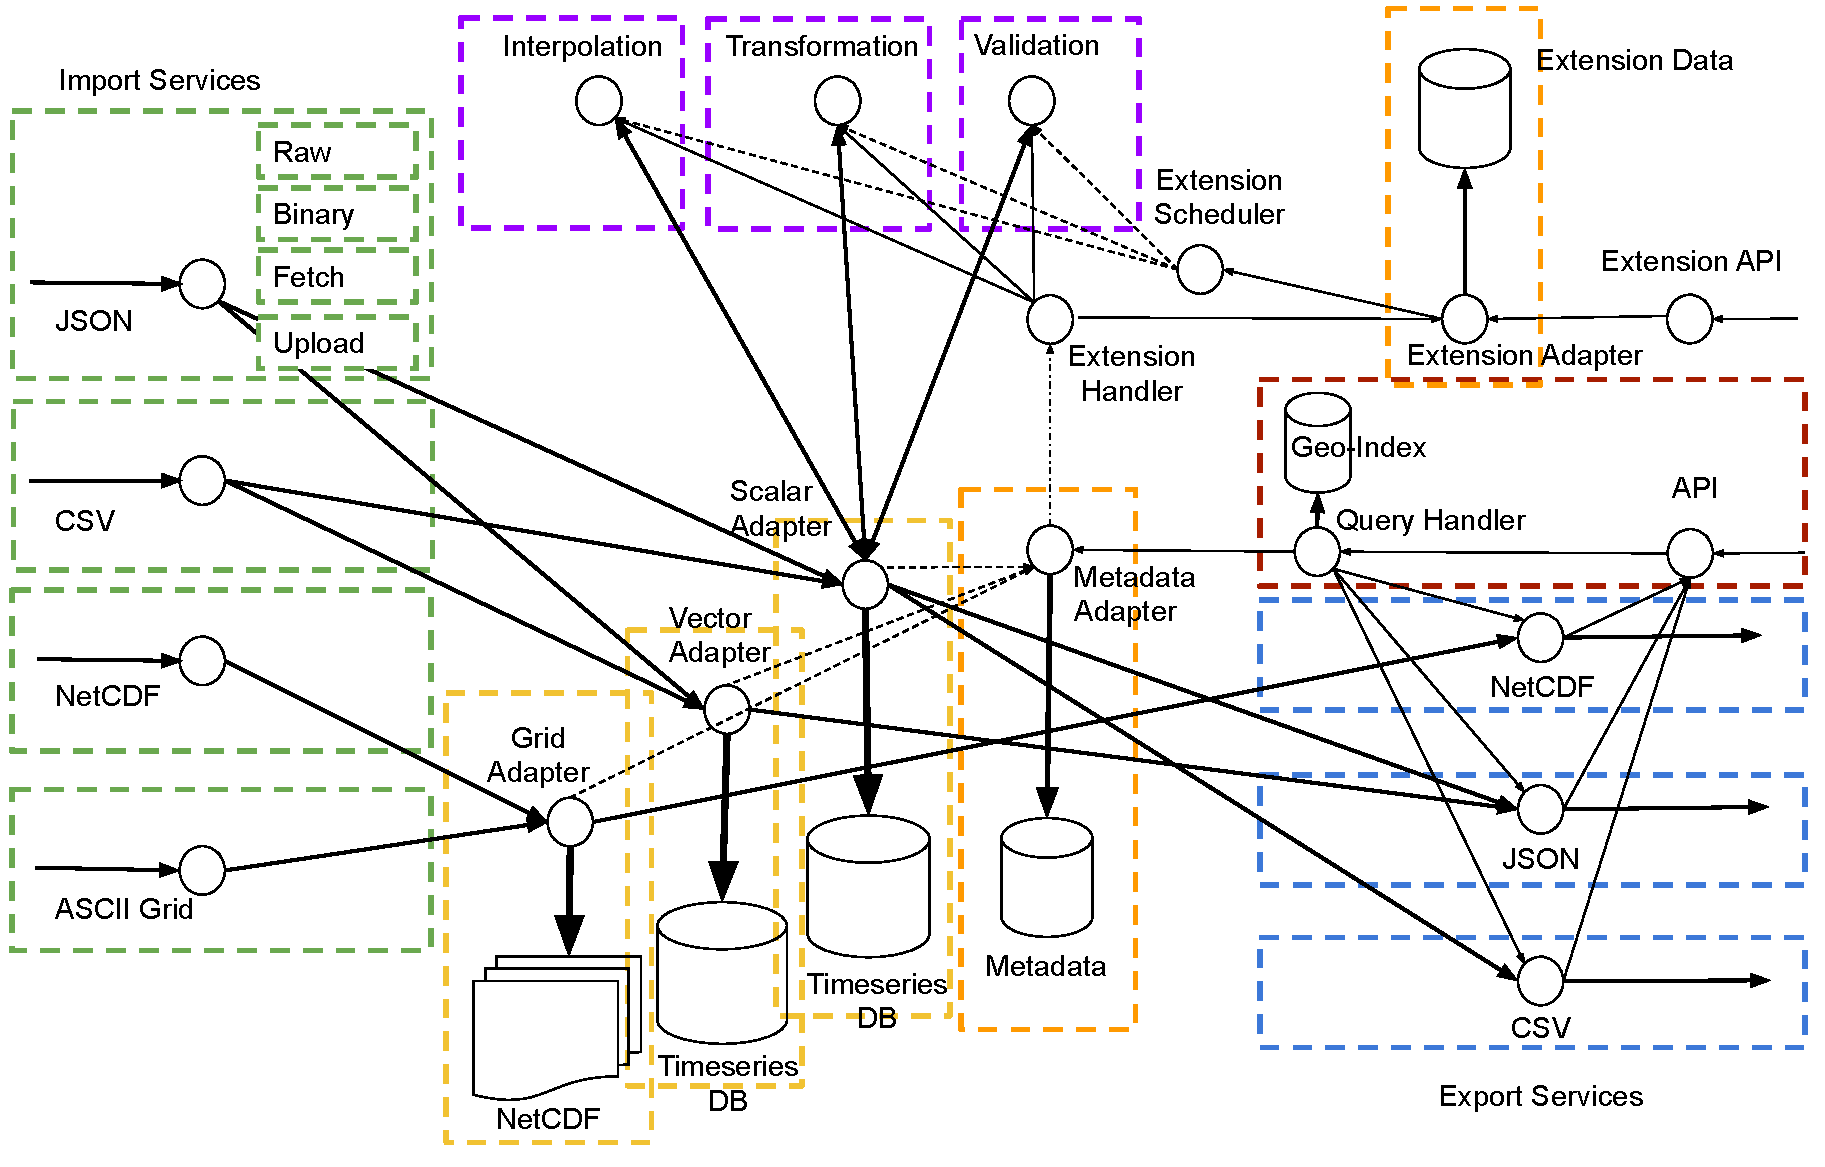
\includegraphics[width=0.5\textwidth]{images/separation_microservices-p1.pdf}}
\caption{Separation of \acrshort{wdias} microservices.}
\label{pfi:microservice_separation}
\end{figure}

\cref{pfi:microservice_separation} shows the separation of \acrshort{wdias}'s modules into the microservices where each circle represents a microservice. All microservices communicate using a RESTful API. Import modules are shown on the left of figure while export modules are shown on the right. \acrshort{wdias} supports importing
and exporting scalar, vector, and grid timeseries data in multiple formats such as JSON, CSV, NetCDF, and ASCII.
Further, users can add new import and export microservices to support different data formats and ingest/egress methods. Each \emph{import microservice} coverts data to a common scalar, vector, or grid format, and forwards them to the relevant data adapter module. For example, \emph{scalar} and \emph{vector} adapters support data in JSON format. Before feeding grid data into the grid adapter, import grid microservices need to transform data into \acrlong{netCDF} format. Each adapter has an its own database instance optimized to store a specific type of data. For example, timeseries metadata is stored in a relational database for faster querying. It is also cached in an in-memory database to provide low-latency access. \emph{Export microservices} provide data to weather models and users while converting them to the desired format. \emph{Extension} modules perform data preprocessing. \emph{Extension adapter} stores metadata required to trigger an extension. While \emph{extension handler} triggers an extension when a new piece of data arrives, \emph{extension} scheduler triggers an extension based on a predefined time schedule. By implementing microservices as containerized applications, we can simplify deployment of modules and enhance platform independence. Further, \acrshort{wdias} uses \acrfull{k8s} \cite{LinuxFoundationProduction-GradeKubernetes} container orchestration platform to auto-scale microservice instances as the workloads varies.

% \begin{figure}[t!]
% \centerline{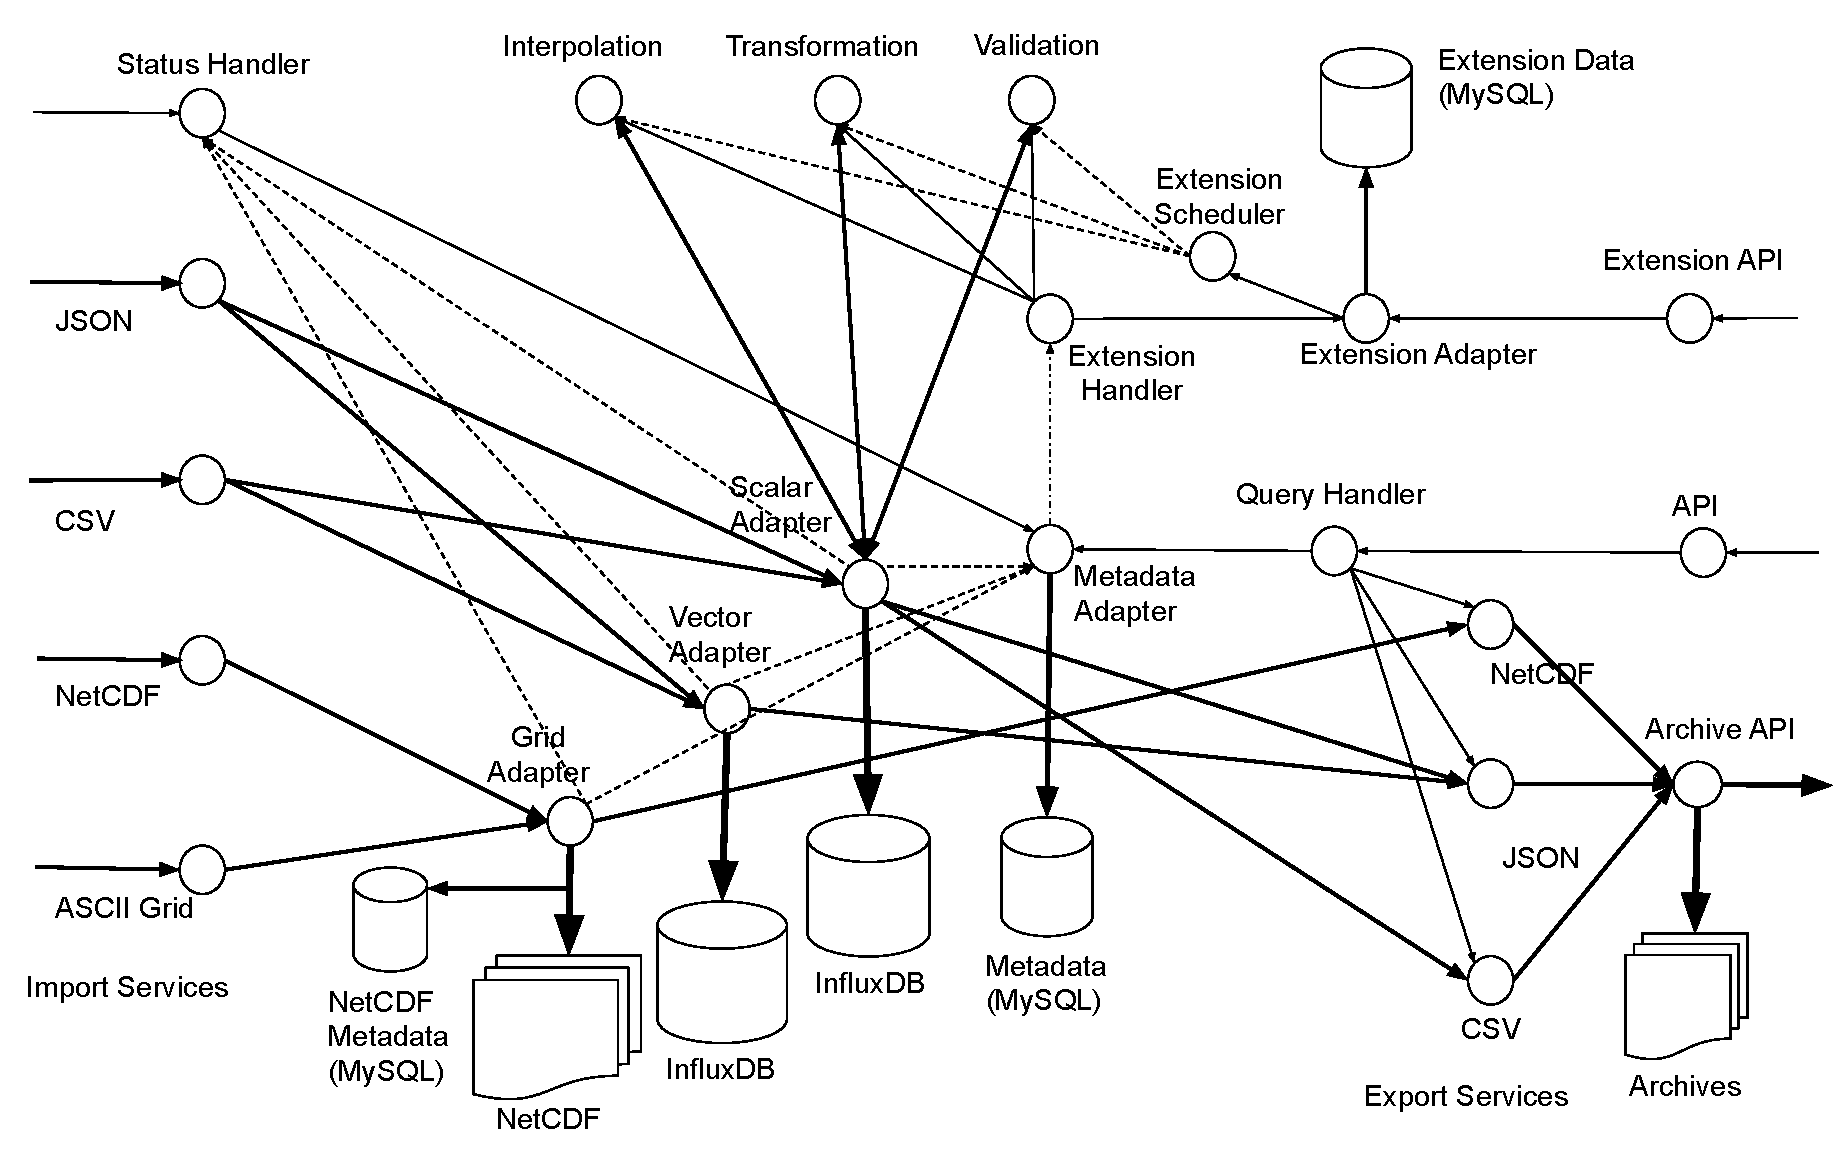
\includegraphics[width=0.5\textwidth]{images/microservice_architecture-handle_on_async-p1.pdf}}
% \caption{Asynchronously handling requests with microservices.}
% \label{pfi:microservice_architecture_async}
% \end{figure}

Each piece of data is tagged with a unique identifier (ID), which is used by all microservices to handle the data. A timeseries is considered as a single piece of data. Ingestion of a large piece of data, such as radar data in \acrshort{netCDF} format, is handled asynchronously. When a request with a large piece of data is received, rather than blocking the request, a unique ID is returned to the caller. This ID can be used later to verify successful processing of data or to download them.
% \db{As shown in \cref{pfi:microservice_architecture_async}, we use a Status Handler to manage the status of asynchronous requests. For example, when an ingestion module receives a large piece of data it is stored on the module. Then the module publishes an event to another service to process it. Once the successful processing of the data is verified, Status Handler updates the system status.}


%%%%%%%%%%%%%%%%%%%%%%%%%%%%%%%%%%%%%%%%%%%%%%%%
\subsection{Database Structure}
\label{psubse:wdias_database}

Timeseries are pervasive in weather domain from observations to forecasting. Thus, \acrshort{wdias} is designed to be data-centric with a special focus on weather timeseries data. Data points in a timeseries can consists of scalar (0D), vector (1D), grid (2D), and polygon (2D) data. We used the following list of metadata to uniquely identify a timeseries:

\begin{itemize}
    \item \texttt{Module ID} -- is the source of data, e.g., weather station ID.
    \item \texttt{Location} -- that the data corresponds to, e.g., point locations and regular or irregular grid locations.
    \item \texttt{Value Type} -- indicates whether data consists of scalar, vector, grid, or polygon values.
    \item \texttt{Parameters} -- indicate the ambient measurements, e.g., temperature and pressure.
    \item \texttt{Timeseries Type} -- indicates whether the data is historical or forecast of a model.
    \item \texttt{Time Step} -- indicates the whether the sampling interval is uniform or not.
\end{itemize}

While a scalar data point consists of a single value, a vector data point consists of two values (e.g., magnitude and the direction of a vector). Whereas a grid data point consists of multiple values. Therefore, to manipulate data efficiently, as seen on \cref{pfi:database_structure} we used a combination of relational, NoSQL, timeseries, and in-memory databases, as well as files. We handle scalar and vector values using two different microservices, namely \textit{adapter-scalar} and \textit{adapter-vector} (see \cref{pfi:microservice_separation}), to isolate performance and faults. We used InfluxDB to manage scalar and vector timeseries data due to its high performance and scalability in handling timeseries data. We used \acrshort{netCDF} files to store grid data as it is the de-factor standard for creating, accessing, and sharing of array-oriented scientific data. To resolve a query targeting timeseries metadata, we need to first identify the source and type of data, as well as where they are stored and what time or geographic range to retrieve. Hence, we used a relational database to manipulate timeseries metadata with low latency. We further used Redis as an in-memory database to enable low-latency query resolution by caching data stored in \textit{adapter-metadata} and \textit{adapter-extension} microservices. Further, spacial indexing (aka., geo-indexing) is needed to support queries based on the geo-location of data which are one of the hardest queries to resolve. Therefore, we used MongoDB, a document-oriented database, to store timeseries metadata as documents for fast retrieval and index searching, as well as to provide geo-indexing for location-based queries.

\begin{figure}[!tb]
\centerline{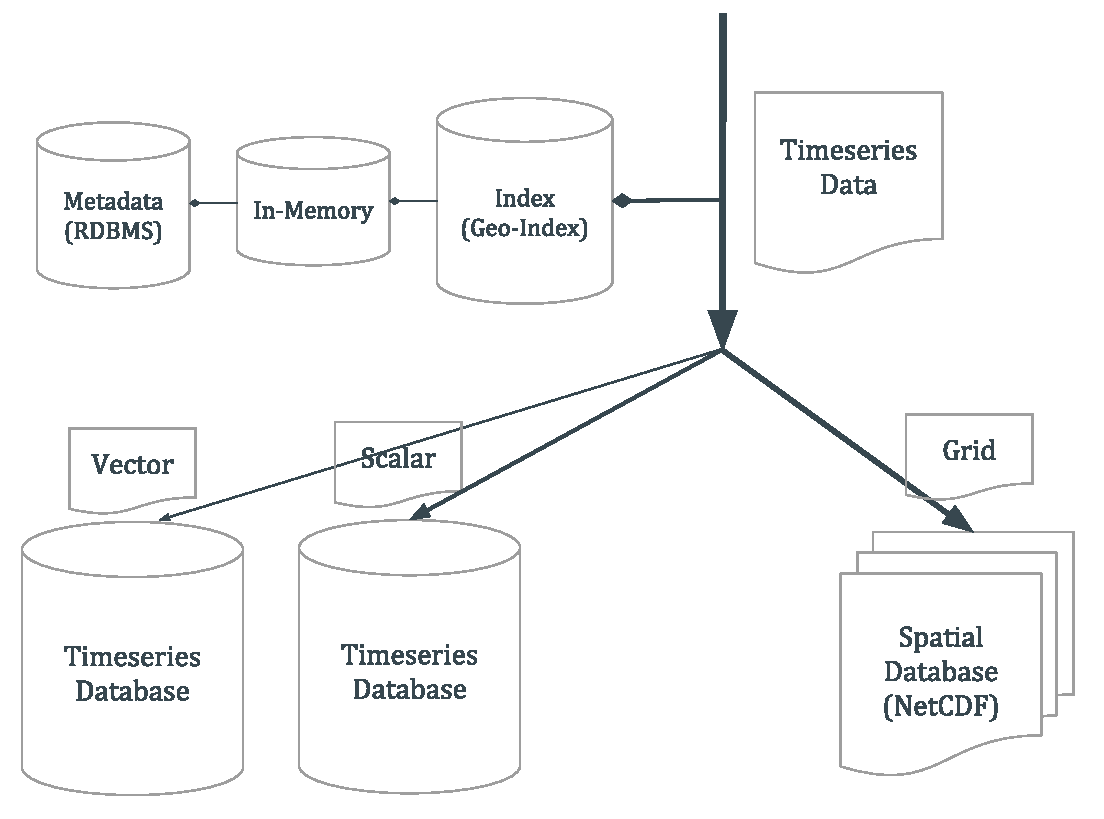
\includegraphics[width=0.4\textwidth]{images/wdias_database_structure_p1.pdf}}
\caption{\acrshort{wdias} database structure.}
\label{pfi:database_structure}
\end{figure}

\acrshort{wdias} supports timeseries and geographic metadata based queries. For example, a query looking for a timeseries in a given area (specified as a polygon in \emph{geoJson} \cite{InternetEngineeringTaskForceGeoJSON} format) could be resolved using geo-indexing. It also supports querying timeseries with a given weather parameter and area, as well as locations within an area of a polygon. While resolving queries made by third-party users, query results include only the unique ID and metadata of timeseries. Subsequently, the user can retrieve the data for the given period by submitting this ID to \emph{export module}.


%%%%%%%%%%%%%%%%%%%%%%%%%%%%%%%%%%%%%%%%%%%%%%%%
\subsection{Data Preprocessing}
\label{psubse:data_preprocessing}

\acrshort{wdias} provides the data preprocessing capabilities via extension modules. As seen in \cref{pfi:summary_weather_data_preprocessing} each extension could be considered as a mathematical function that takes \texttt{p} timeseries variables as input and output \texttt{n} timeseries variables. As seen on bottom half of figure, these functions are typically used for data quality checks, interpolation (both serial and spatial), and transformation. To further extend the function at run time without creating a new module, the \textit{bind constant} can be set at the time of creating a trigger for an extension. For example, such features are needed as we may need to generate two different timeseries by sub-sampling 1-minute data to 5 minutes and one hour. While this increases the data stored by \acrshort{wdias}, it reduces the computational time as NWMs can readily use the data without transforming them at the run time. \cref{pli:extension_triggers} shows the format of a request made to update an extension at the time of triggering it. Each extension trigger needs to have a unique ID (line 2). Then the user can define the extension type and the microservice responsible of processing it (lines 3 and 4). Using lines 5-12 the user can map timeseries into input variable \emph{X} and output variable \emph{Y} as seen in \cref{pfi:summary_weather_data_preprocessing}. Finally, user can also define when to trigger the extension (e.g., \textit{OnChange} or \textit{OnTime}) and any options such as bind constant. Using different update requests \acrshort{wdias} can create multiple triggers for an extension. When the trigger is set as \emph{OnChange}, the \emph{extension handler} triggers the registered extension when new data are ingested into the timeseries. Whereas the \emph{extension scheduler} triggers the registered extension when the trigger is set as \emph{OnTime}. 


\begin{figure}[!tb]
\centerline{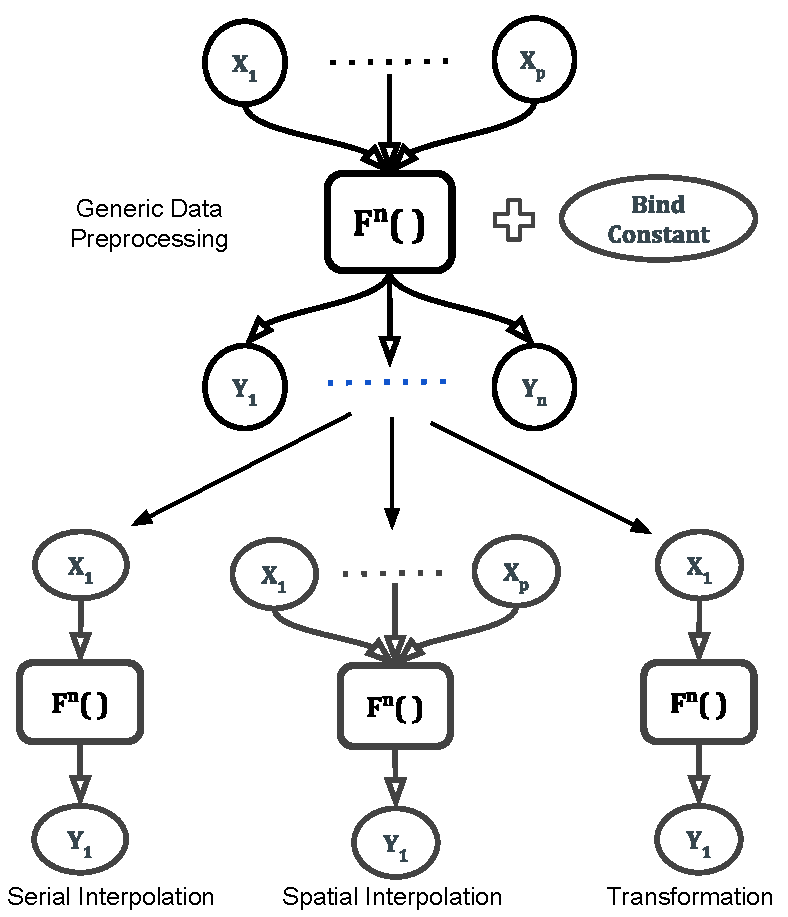
\includegraphics[width=0.375\textwidth]{images/summary_weather_data_preprocessing_p1.pdf}}
\caption{Functional approach to weather data preprocessing.}
\label{pfi:summary_weather_data_preprocessing}
\end{figure}

\begin{minipage}{0.47\textwidth}
\begin{lstlisting}[language=Python, caption=Format of a request made to update an extension., label=pli:extension_triggers]
{
    "extensionId": "", //Trigger unique ID
    "extension": "Interpolation | Transformation | Validation",
    "function": "", //Mapping microservice
    "variables": [ //Map timeseries to variables
        {
            "variableId": "",
            "metadata/metadtaIds": {...}
        } 
    ],
    "inputVariables": [], //Input timeseries
    "outputVariables": [], //Output timeseries
    "trigger": [ // When to trigger the function
        {}
            "trigger_type": "OnChange | OnTime",
            "trigger_on": []
        }
    ],
    "options": { //Run time bind constant data
    }
}
\end{lstlisting}
\end{minipage}


%%%%%%%%%%%%%%%%%%%%%%%%%%%%%%%%%%%%%%%%%%%%%%%%
%\subsection{Query Resolution}
%\label{psubse:query_timeseries}

% \begin{lstlisting}[caption=Geo search timeseries, label=pli:geo_search]
%     POST <HOST_NAME>/query/timeseries
%     JSON Body:
%     {
%         "geoJson": {
%             "type": "Polygon",
%             "coordinates": [
%                 [
%                     [<longitude>, <latitude>],
%                     ...
%                 ]
%             ]
%         }
%     }
% \end{lstlisting}



%%%%%%%%%%%%%%%%%%%%%%%%%%%%%%%%%%%%%%%%%%%%%%%%%%%%%%%%%%%%%%%%%%%%%%%%%%%%%%%%
\section{Performance Analysis}
\label{pse:performance_analysis}

%%%%%%%%%%%%%%%%%%%%%%%%%%%%%%%%%%%%%%%%%%%%%%%%
\subsection{Experimental Setup}
\label{psubse:experimental_setup}

As a weather data integration and assimilation system is expected to handle variety of data sources and types, we created a synthetic workload consisting of 70\% scalar, 20\% vector, and 10\% grid values. 
We created 1,000 timeseries using 30-day traces from five weather stations of \acrlong{curw}. Locations of timeseries were set based on the Google's Countries dataset with 250 locations \cite{GoogleGoogleCounties}. 
For each location we created four timeseries by varying the source of data (i.e., \texttt{Module ID}) to create a total of 1,000 timeseries. Weather data for a day was included in a single request, and a date counter was used to keep track of the day. For each day, scalar timeseries randomly picked precipitation data from one of the five weather stations. Once 30 days are reached, we go back to the first date of trace and continued again. Similarly, vector timeseries randomly picked wind speed and direction data from one of the weather stations. To create grid data, we considered a 2D regular grid of $120 \times 139$. 
We created 100 grid timeseries using 30-day traces from simulated water levels which produced ASCII grid files.
Therefore, while scalar and vector data points contained a single value for a timestamp, a grid data point contained $120 \times 139$ values. Thus, grid data are much more difficult to handle compared to scalar and vector data.

Load testing was performed using Apache JMeter with distributed testing feature, which use multiple workload generators to create a high throughput workload. For both insert and retrieve requests, we varied the request size by varying the number of data points per request. For example, we insert/request data for an entire day at 60, 30, and 15 min resolutions. For a given request size, we issued requests at different rates such as 10, 50, 100, 200, and 300 requests per second. For each request size, we ran a separate load test while increasing the request rate from 10 to 300 within 30 min.  After reaching the highest request rate, we also measured how the system would gradually release the resources when there is no load on the system. \gk{We also performed geo-search queries to measure the performance of the query resolution. The test case gets all the locations near to request timeseries' actual location and check whether timeseries location exists among them. Then get the timeseries available in the given location}.
\dbc{I think my fix now cover Insert and Retrieve. But we still need to talk about Query.}
\gkc{Updated}


% \acrshort{wdias} was deployed using \acrfull{eks} container orchestration platform. \cref{ptab:aws_eks_nodes} shows the list of nodes used in the experimental setup. \db{\emph{Core} node executed metadata, extensions, query, status and extension microservices. Whereas the \emph{grid} node executed the grid adapter, as well as grid data import and export services. Scalar and vector adapters, as well as scalar and vector import and export services were deployed on the \emph{scalar} node. JMeter and metric server executed on the \emph{test} node.} Given a set of computing resources, to get the better performance, we scheduled each microservice on a predefined set of nodes.
\acrshort{wdias} was deployed using \acrfull{eks} container orchestration platform. \cref{ptab:aws_eks_nodes} shows the list of nodes used in the experimental setup. The metadata, extensions, query, status and extension microservices scheduled to host on the core labeled node. The grid adapter, as well as grid data import and export microservices scheduled to host on grid labeled node due to those services are closely communicating to each other. Scalar and vector adapters, as well as scalar and vector import and export services were deployed on the scalar labeled node due to closely communication. Then JMeter test servers hosted on test labeled nodes separately, since those want high network usage to connect with the \acrshort{wdias} system.
\dbc{Some of the terms in highlighted part was never mentioned in text. Hence, it's important that these are introduced in Sec. II.A}
\gkc{Reworded}

% \db{WDIAS, uses the Concurrency Thread Group with Throughput Shaping Timer because it supports the open workload approach.}
\dbc{Highlighted sentence is not clear to me.}

% \begin{itemize}
%     \item \emph{closed system model} \cite{Haggett1998AnWales} -- a new request is only triggered by the completion of a previous request, following by a think time.
%     \item \emph{open system model} -- new requests arrival independently of completions.
% \end{itemize}
\dbc{What are these?}
\gkc{It need too much details for the explanation. No need for the paper I think.}
\dbc{From Table II to V it seems we separated out timeseries and grid requests. Also, there are Insert, Retrieve, and query requests. These need to be clearly mentioned in this sub-section to avoid any confusion.}

\begin{table}[tb!]
\caption{\acrshort{eks} nodes}
\begin{center}
\begin{adjustbox}{width=0.45\textwidth}
\begin{tabular}{|l|r|r|r|r|l|}
\hline
\textbf{Node Label} & \textbf{vCPUs} & \textbf{RAM (GB)} & \textbf{Storage (GB)} & \textbf{Quantity} & \textbf{EC2 Name} \\ \hline
core & 16 & 32 & 15 & 1 & c5.4xlarge \\ \hline
grid & 8 & 16 & 25 & 1 & c5.2xlarge \\ \hline
scalar & 8 & 16 & 20 & 1 & c5.2xlarge \\ \hline
test & 4 & 10.5 & 5 & 1 & c5n.xlarge \\ \hline
\end{tabular}
\end{adjustbox}
\label{ptab:aws_eks_nodes}
\end{center}
\end{table}


%%%%%%%%%%%%%%%%%%%%%%%%%%%%%%%%%%%%%%%%%%%%%%%%
\subsection{Performance Evaluation}
\label{psubse:performance_evaluation}

\cref{ptab:obs_all_60_min_summary_throughput} to \cref{ptab:obs_all_15_min_summary_throughput} show the throughput (measured as \acrlong{rps}), latency, and errors under three different data resolutions with a fixed service setup. Whereas \cref{ptab:obs_all_auto_15_min_summary_throughput} shows the performance with the container auto-scaling. It can be seen that each test resulted in approximately 310K requests within 30 minutes. Avg., 90\%, and STD indicates the average, standard deviation, and 90\% percentile for latency.  Other than some grid timeseries inserts, all other operations succeed with no errors.

\dbc{What's the request rate when collecting data for Tables II to V?}
\gkc{I removed the graph based on your suggestion: performance\_study\_v4.pdf}
\dbc{It seems you are using RPS to indicate throughput, which is the rate that we make requests not the rate that system responds. However, if latency is low and requests don't pile up we can say system can handle this request rate. We need to be a bit clear on this.}
\gkc{Okay, Thanks for clearing it out}

From \cref{ptab:obs_all_60_min_summary_throughput} to \cref{ptab:obs_all_15_min_summary_throughput} it can be seen that the average and 90\% percentile latency to insert scalar and vector timeseries increased by 2 ms and 10 ms, respectively as we increase the request size. Still \acrshort{wdias} was able to accept 40.5 \acrshort{rps}. However, while retrieving the scalar and vector timeseries data, latency got doubled while handling the 15-min data compared to 30-min data. \db{This is due to heavy writes on the timeseries database, at the same time trying to retrieve data.} However, there is no noticeable reduction in RPS. Therefore, even through the data volume increased by four times, \acrshort{wdias} performance degradation is sub-linear. 

\dbc{How come heavy writing happens when retrieving data? Shouldn't it happen during ingestion. Or is it because we are running data preprocessing at the time of request? This need to be clearly explained.}
\gkc{I meant all read and writes happens in a single database. So the db writes affects on db reads}

\begin{table}[tb!]
\centering
\caption{Performance while processing 60-min data requests.}
\begin{adjustbox}{width=0.45\textwidth}
% \footnotesize
\begin{tabular}{|l|r|r|r|r|r|r|}
\hline
\textbf{Request Type} & \textbf{\# Samples} & \textbf{RPS} & \textbf{Avg.} & \textbf{90\%} & \textbf{STD} & \textbf{Error \%} \\ \hline
Insert Timeseries & 71826 & 40.5 & 28 & 31 & 58.74 & 0.00\% \\ \hline
Retrieve Timeseries & 71796 & 40.7 & 8 & 10 & 4.18 & 0.00\% \\ \hline
Insert Grid & 7982 & 4.5 & 23 & 26 & 4.23 & 0.06\% \\ \hline
Retrieve Grid & 7979 & 4.5 & 68 & 75 & 10.11 & 0.00\% \\ \hline
Query Location & 71804 & 40.5 & 3 & 3 & 1.52 & 0.00\% \\ \hline
\textbf{TOTAL} & 311182 & 175.4 & 127 & 503 & 207.80 & 0.00\% \\ \hline
%\multicolumn{4}{l}{$^{\mathrm{a}}$S.D.: Standard Deviation}{$^{\mathrm{b}}$90\%: 90\% percentile}
\end{tabular}
\end{adjustbox}
\label{ptab:obs_all_60_min_summary_throughput}
\end{table}

\dbc{We need to use a more meaningful term than ``60-min data'', ``30-min data', and ``15-min data'' because these reflect only the size of Retrieve requests. If this also indicates Insert timeseries' sampling interval, we need to clearly mention this in Sec. III.A}
\gkc{Agreed. Better to come up with a new terminology. Reword to make it more clear.}

\begin{table}[tb!]
\caption{Performance while processing 30-min data requests.}
\begin{center}
\begin{adjustbox}{width=0.45\textwidth}
% \footnotesize
\begin{tabular}{|l|r|r|r|r|r|r|}
\hline
\textbf{Request Type} & \textbf{\# Samples} & \textbf{RPS} & \textbf{Avg.} & \textbf{90\%} & \textbf{STD} & \textbf{Error \%} \\ \hline
Insert Timeseries & 71759 & 40.5 & 29 & 32 & 50.97 & 0.00\% \\ \hline
Retrieve Timeseries & 71730 & 40.6 & 9 & 10 & 6.04 & 0.00\% \\ \hline
Insert Grid & 7972 & 4.5 & 44 & 49 & 8.17 & 0.08\% \\ \hline
Retrieve Grid & 7971 & 4.5 & 81 & 93 & 15.15 & 0.00\% \\ \hline
Query Location & 71734 & 40.5 & 3 & 3 & 1.90 & 0.00\% \\ \hline
TOTAL & 310878 & 175.3 & 129 & 0 & 207.10 & 0.00\% \\ \hline
%\multicolumn{4}{l}{$^{\mathrm{a}}$S.D.: Standard Deviation}{$^{\mathrm{b}}$90\%: 90\% percentile}
\end{tabular}
\end{adjustbox}
\label{ptab:obs_all_30_min_summary_throughput}
\end{center}
\end{table}

Latency to insert grid timeseries data is relatively low compared to scalar or vector inserts as grid data are handled asynchronously, and before processing data the request handler store the grid files upload via a single thread. When the number of grid files doubled, latency also doubled as \gk{the request handler needs to store twice the data before}. \db{Yet, \acrshort{wdias} was able to handle the all the incoming requests. The error rate increased because, randomly some request handlers having deadlocks while storing the grid data and we used 10 seconds timeout for request to avoid pile up requests in the JMeter. When a request timeout happens, it consider as an error.}
\dbc{We need to talk about why errors increased.}
\gkc{Added}
\dbc{Explain why when the number of grid files double, latency also double. Is it because twice the bandwidth is needed?}
\gkc{Updated}
\db{Retrieving of Grid timeseries data happens on demand with the current \acrshort{wdias} implementation. But it is possible to upgrade the system to support asynchronously download alongside with direct download. Also while download the data, the grid data need to be extract from netCDF files which is a costly operation. Because of these, the latency of download the the Grid data is bit higher than the other test cases.}
\dbc{Highlighted text is not clear to me. Also, I'm confused about how asyn cases are handled for Insert and Retrieve. Did you measure latency to get only the unique ID or entire data?}
\gkc{Measure the latency for get entire data. For insert grid timeseries data, I handle it async. But for retrieve grid timeseries, I'm not handling them async (but we can update the system to do so). If the user know the unique ID of the timeseries, he can request to get grid data within provided time interval such as get grid data for a given day.}

\begin{table}[tb!]
\caption{Performance while processing 15-min data requests.}
\begin{center}
\begin{adjustbox}{width=0.45\textwidth}
% \footnotesize
\begin{tabular}{|l|r|r|r|r|r|r|}
\hline
\textbf{Request Type} & \textbf{\# Samples} & \textbf{RPS} & \textbf{Avg.} & \textbf{90\%} & \textbf{STD} & \textbf{Error \%} \\ \hline
Insert Timeseries & 71775 & 40.5 & 30 & 41 & 51.71 & 0.00\%  \\ \hline
Retrieve Timeseries & 71736 & 40.6 & 23 & 32 & 50.18 & 0.00\%  \\ \hline
Insert Grid & 7975 & 4.5 & 91 & 112 & 19.58 & 1.42\% \\ \hline
Retrieve Grid & 7972 & 4.5 & 118 & 165 & 56.15 & 0.00\% \\ \hline
Query Location & 71749 & 40.5 & 3 & 4 & 2.32 & 0.00\% \\ \hline
\textbf{TOTAL} & 310934 & 175.4 & 134 & 503 & 206.40 & 0.04\% \\ \hline
%\multicolumn{4}{l}{$^{\mathrm{a}}$S.D.: Standard Deviation}{$^{\mathrm{b}}$90\%: 90\% percentile}
\end{tabular}
\end{adjustbox}
\label{ptab:obs_all_15_min_summary_throughput}
\end{center}
\end{table}

In all test cases, performance in resolving location-based queries remained the same. This was due to the geo-index build using the NoSQL database. 
\dbc{When we change from 1H to 15min, was there any impact on location queries? My understanding is there no such change unless queries were issued more frequently (this seems to be not the case from 3 tables) or queries asked for more data?}
\gkc{No impact on location queries when change from 1H to 15min. But internally system get timeseries metadata for insertions. I removed separate load testing on queries, because of too much content.}
% To get better performance test on the query module, we performed set of complex queries as shown in the \cref{ptab}

\begin{table}[tb!]
\caption{Performance while processing 60-min data requests when auto-scaling is enabled.}
\begin{center}
\begin{adjustbox}{width=0.45\textwidth}
\footnotesize
\begin{tabular}{|l|r|r|r|r|r|r|}
\hline
\textbf{Request Type} & \textbf{\# Samples} & \textbf{RPS} & \textbf{Avg.} & \textbf{90\%} & \textbf{STD} & \textbf{Error \%}\\ \hline
Insert Timeseries & 71727 & 40.5 & 34 & 27 & 118.78 & 0.00\% \\ \hline
Retrieve Timeseries & 71693 & 40.5 & 7 & 9 & 18.72 & 0.00\% \\ \hline
Insert Grid & 7968 & 4.5 & 87 & 98 & 14.07 & 0.18\% \\ \hline
Retrieve Grid & 7965 & 4.5 & 89 & 110 & 37.79 & 0.00\% \\ \hline
Query Location & 71704 & 40.5 & 1 & 2 & 2.05 & 0.00\% \\ \hline
\textbf{TOTAL} & 310734 & 175.3 & 130 & 501 & 212.35 & 0.00\% \\ \hline
%\multicolumn{4}{l}{$^{\mathrm{a}}$S.D.: Standard Deviation}{$^{\mathrm{b}}$90\%: 90\% percentile}
\end{tabular}
\end{adjustbox}
\label{ptab:obs_all_auto_15_min_summary_throughput}
\end{center}
\end{table}

\cref{ptab:obs_all_auto_15_min_summary_throughput} shows the performance when we enabled container auto-scaling. When we were inserting and retrieving data at 15-min resolution, microservices handling grid data had high resource utilization and 1.4\% of the grid insert requests failed. Once the auto-scaling was enabled, resource utilization of microservices were balanced. This reduced both the errors (0.18\%) and the overall latency for inserting and retrieving grid data.

\begin{figure}[!tb]
\centerline{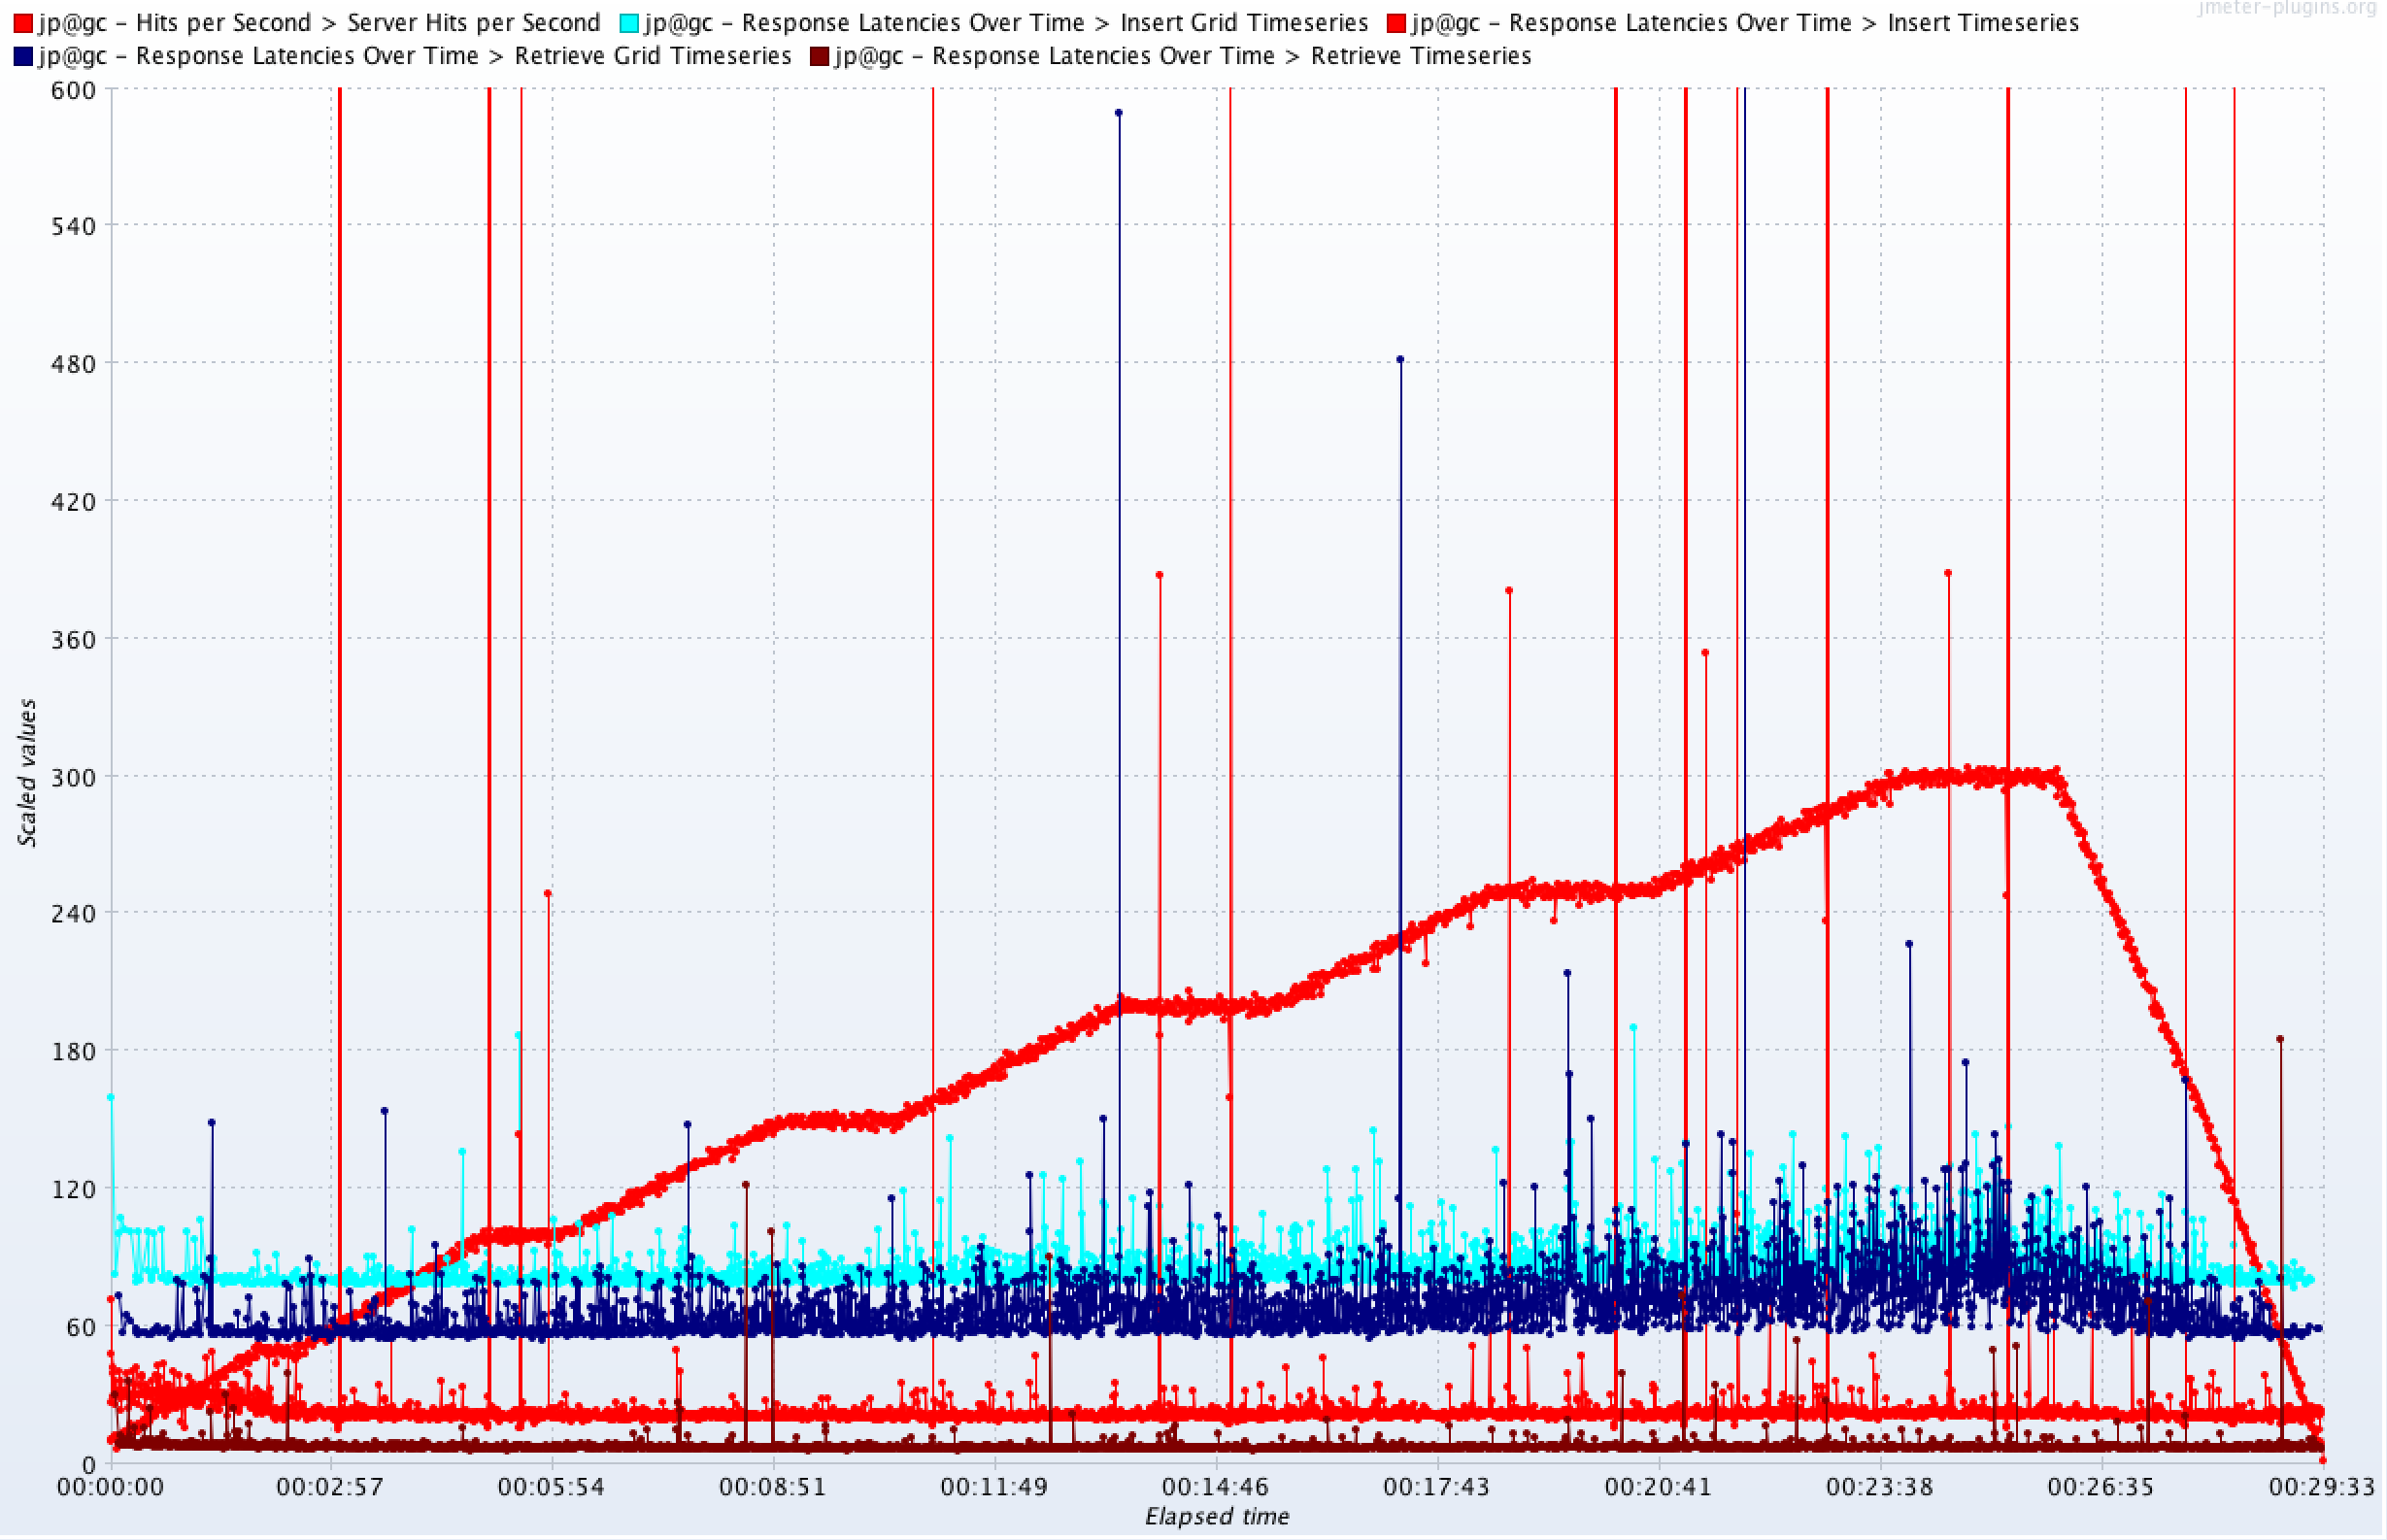
\includegraphics[width=0.5\textwidth]{results/obs/all_auto/obs_all_auto_15m_res_latencies_against_hits.png}}
\caption{Variation of request rate and latency with elapsed time with auto-scaling and 15-min data.}
\label{pfi:test_obs_auto_all_15_min_latency_vs_hits}
\end{figure}

\cref{pfi:test_obs_auto_all_15_min_latency_vs_hits} shows the latency of each request type under 15-min resolution and auto-scaling. Even through the request rate increased linearly (indicated by red line), no significant increase in latency was observed for request types other than grid data related requests (indicated by blue line). Even then, latency was within $2\times$ while the request rate was $5\times$.

%\begin{figure}[!tb]
%\centerline{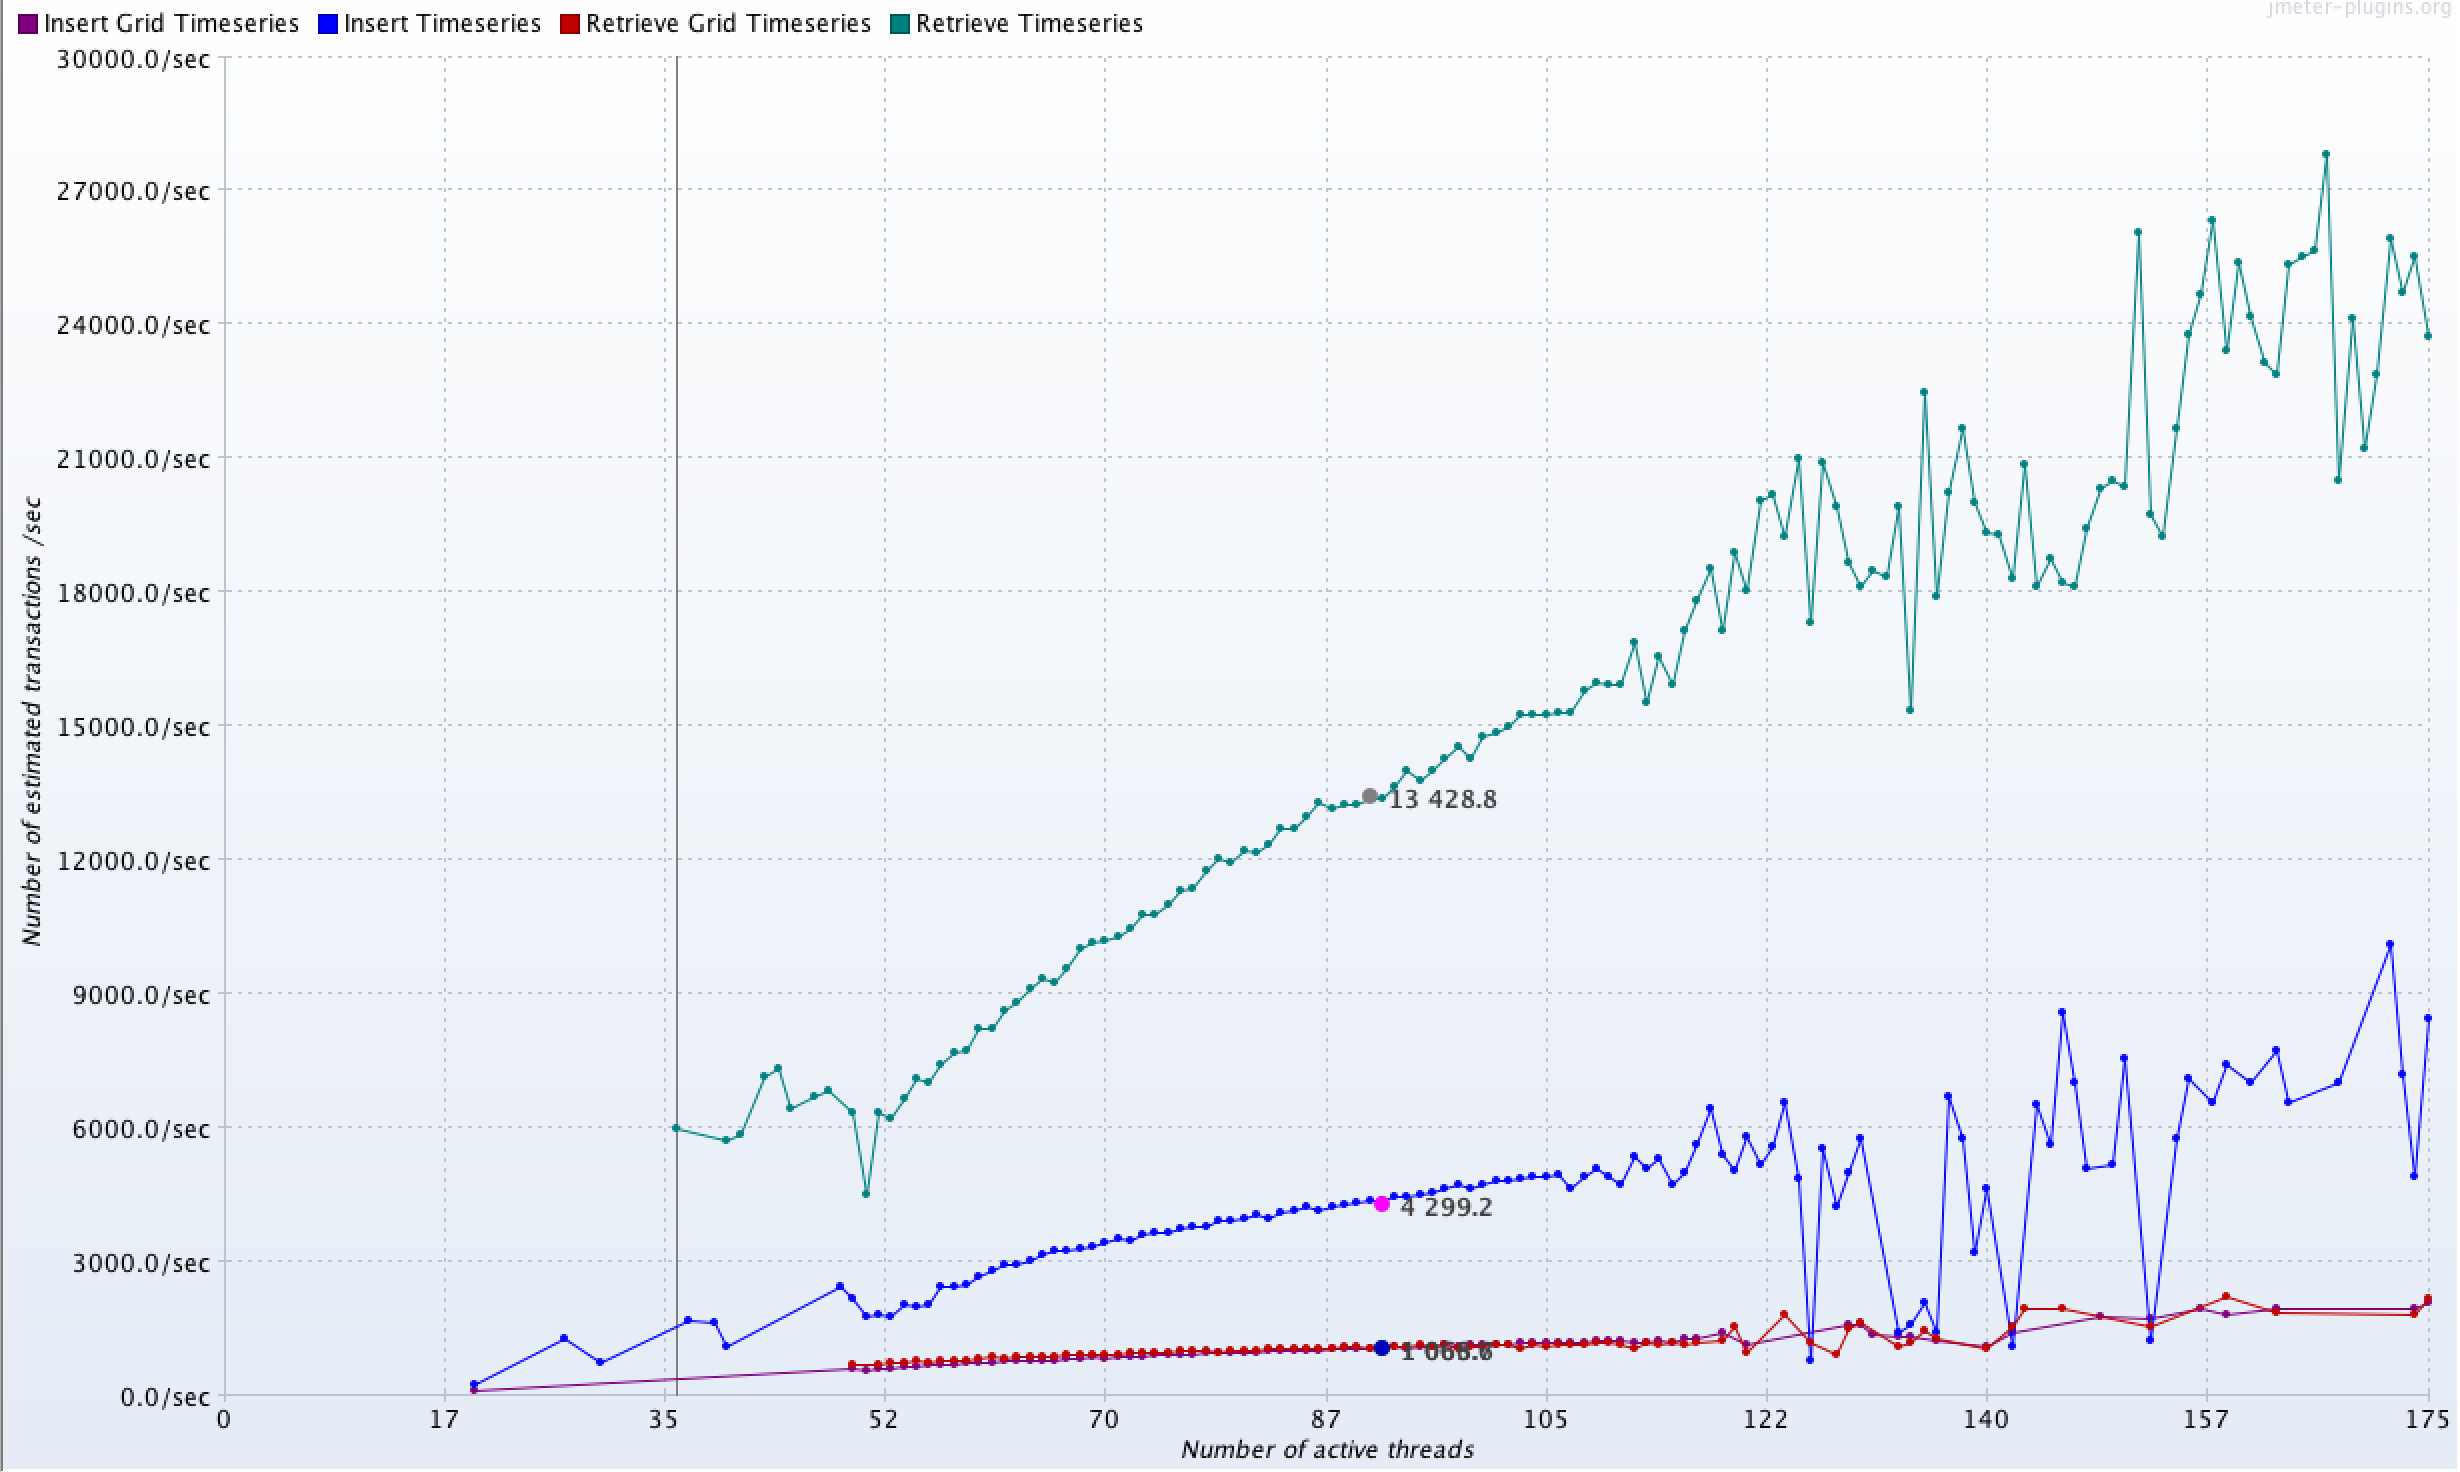
\includegraphics[width=0.5\textwidth]{results/obs/all_auto/obs_all_auto_15m_transaction_throughtput_vs_threads.png}}
%\caption{Transnational throughput vs number of active threads while performance test with 15min data and auto-scaling enabled.}
%\label{pfi:test_obs_auto_all_15_min_throughput_vs_threads}
%\end{figure}

%\cref{pfi:test_obs_auto_all_15_min_throughput_vs_threads} shows the total server's transaction throughput against the number of active threads.
%The formula for total server transaction throughput is \(<active threads> * 1 second / <1 thread response time>\) \cite{JMeterPluginsTransactionPlugin}. It shows the statistical maximum possible number of transactions based on the number of users accessing the application.
%By combining the \cref{pfi:test_obs_auto_all_15_min_latency_vs_hits}, this graph shows that the throughput of the system gets increased without much change in the latency, thus it proves the scalability of the \acrshort{wdias}.
\dbc{I'm removing Fig. 7 as it's a forecast not actual results. Ok to keep this in thesis.}
\gkc{Agreed}

\begin{figure}[!tb]
    \centering
    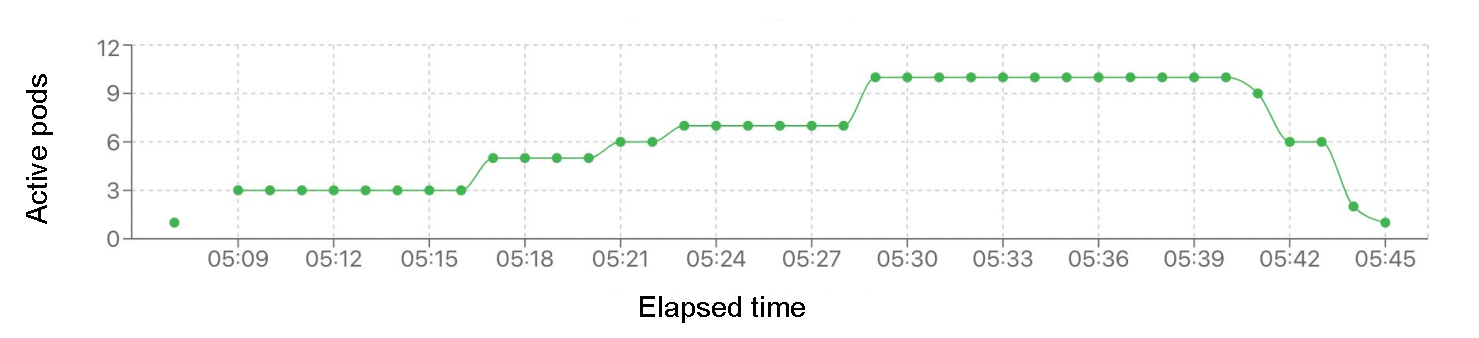
\includegraphics[width=0.5\textwidth]{images/obs_all_auto_15m_import_ascii_pods_p1.pdf}
    \caption{Number of running replicas of import ascii grid microservice over time with auto-scaling enabled.}
    \label{pfi:obs_all_auto_15m_import_grid_pod}
\end{figure}

\dbc{x and y axis of \cref{pfi:obs_all_auto_15m_import_grid_pod} need to be labelled}
\gkc{Updated}

As the performance bottleneck was mostly on microservices handing grid data, in \cref{pfi:obs_all_auto_15m_import_grid_pod}, we look at how the number of \textit{import ascii grid} pods are scheduled with time. \gk{In \acrshort{k8s}, a running containerized application called as a pod}. We configured the \acrshort{k8s} for \textit{import ascii grid} microservice to horizontal scale up to maximum ten pods with a CPU utilization threshold of 80\%. A new pod was allowed to initiate with a single virtual CPU (vCPU) and was able to scale up to two vCPUs per pod. As shown in the graphs, three pods were scheduled initially as per the configuration of \acrshort{k8s}. As the workload increased, a new pod was spawned when the average CPU utilization reached 80\%. Once the 10 pods were reached no new pods were spawned. Pods were also able to scale vertically up to two vCPUs. From the 0.18\% failed insert grid data operations, most of them were caused once the ten pod and 2 vCPUs per pod limit was reached. It was further noted that once the workload is cut off, the system gradually reduces the number of pods and reach the minimum  configured number of pods.
\dbc{Up to this point we didn't use the word pod. Would it be better to stick to word containers? Also, we never talked about a helm chart.}
\gkc{Introduced the word ''pod''. Removed helm chart.}
\dbc{Either in Sec II.B or III.A we need to briefly mention that grid operations are difficult to handle compared to scalar and vector.}
\gkc{Mentioned in III.A}
\dbc{import-ascii-grid-upload was never mentioned}
\gkc{Changed as ''import ascii grid'' microservice}

%%%%%%%%%%%%%%%%%%%%%%%%%%%%%%%%%%%%%%%%%%%%%%%%
% \subsection{Performance Metrics Analysis}
% \label{psubse:performance_metrics}

%The \emph{Latency} for each operation type kept constant over the whole test plan run time without any significant change. When the request size increased from 24 data points to 96 data points, the latency increase throughout the whole test plan with a smaller number. But for each test run, the latency kept constant over time.
%During the \cref{ptab:obs_all_auto_15_min_summary_throughput} test run, the performance of the Grid data got better when compared to \cref{ptab:obs_all_15_min_summary_throughput}. This means by adding more resources to the \acrshort{wdias}, it can handle more workload on the system.

%While keeping the latency constant without significant change, the \emph{throughput} of the \acrshort{wdias} kept constant while increasing the request size from 60min data (24 data points) to 15min data (96 data points) for all the data types such as Scalar, Vector, and Grid.
%When the number of active threads increased, the \acrshort{wdias} able to provide the same throughput with maintaining the latency stable.

%When looking into the \emph{resource utilization} of \acrshort{wdias}; since it is using the \acrshort{k8s} as the container orchestration system, it allows us to scale up and cool down the system as required based on the workload. This demonstrates the test plan of \cref{ptab:obs_all_15_min_summary_throughput}, and the system gets scale up to the maximum at the peak time. Then cool down to a single pod after finishing the test cases.
%Given above \acrshort{wdias} can run from 1 CPU node to nodes with 100 CPUs. As described in the \cref{pse:wdias_architecture}, it uses many of the concepts of modern microservice architecture to create stateless, failover, redundant microservice to achieve such capabilities.

%The \acrshort{wdias} supports \emph{auto scaling} by out of the box with \acrshort{k8s}. Services can configure with a maximum number of pods to avoid over resource usage. When there is not much workload on the system, the system cools down to fewer pods to save more resources. When there is an issue with a pod, \acrshort{k8s} auto-schedule another pod and remove the unhealthy pod. Also, it allows updating the system without any downtime with rollback updates.

%\emph{Risk of unable to process data} during the test performance, the \acrshort{wdias} processed many requests with higher request size than the normal usage with a lower rate of failures to process the requests, mainly with insert Grid data. If the usage of \acrshort{wdias} wants to reduce the risk of unable to process data, then the system can configure to run with redundant pods to handle spike of workloads. Also while configuring for the auto-scaling, the \acrshort{k8s} can configure to maintain a lower amount of CPU usage such as 50\% to 60\% rather than 80\%. Such configuration with always spawn new pods to handle double of current peak load.

%%%%%%%%%%%%%%%%%%%%%%%%%%%%%%%%%%%%%%%%%%%%%%%%%%%%%%%%%%%%%%%%%%%%%%%%%%%%%%%%
\subsection{Discussion}
\label{psubse:discussion}

As observed from above analysis \acrshort{wdias} could handle increasing workloads (in terms of both the request rate and request size) in a salable manner without a significant increase in latency or errors. It was further noted that auto-scaling containers lead to better performance at a reduced cost. \acrshort{wdias} has several other features/properties that is not covered under above analysis. For example, the extension module enables various prepossessing modules to be integrated into the system as plugins.
With large-scale container orchestration, \acrshort{wdias} can be made to scale from a single vCPU node to nodes with 100s of vCPUs. Moreover, due to the microservices architecture, \acrshort{wdias} can create stateless and redundant modules with failover capabilities. For example, when there is an issue with a pod, container orchestration platform could auto-schedule another pod. Furthermore, microservices allow updating the system without any downtime \gk{such that deploy update application first, and forward the request after running enough pods successfully. In case of failures, the system rollback to previous successfully running version}.
\dbc{Is ``rollback updates'' a standard word?}
\gkc{Reword}
\dbc{While performance testing didn't we run in preprocessing modules? If so, it need to be clearly mentioned}
\gkc{Yes, I did not check the performance of preprocessing modules. Where should I update the it? In III.C or III.B?}

\gk{For each scalar and vector data, the system uses a separate InfluxDB database for gain more performance. Even with each data type uses a single instance to avoided potential data consistency issues, it also constrained the throughput and increased the latency. But somewhat high variability in insert and retrieval operations was due to high read/write operation on each database instance.} Due to the microservices architecture it is possible to easily extend \acrshort{wdias} to support high availability with timeseries database by using sharding and replication features (e.g.,InfluxDB Enterprise edition).
Further the use of files for netCDF affected the performance of grid data related requests. As microservices can be written in any programming language, more computationally heavy modules such as \acrshort{netCDF}-based grid data processing functions could be written using C or FORTRAN \acrshort{netCDF} wrapper as opposed to Python \acrshort{netCDF} wrapper.
\dbc{one InfluxDB for both or one each?}
\gkc{each one has separate influxdb instance. I think it also clear in \cref{pfi:database_structure}. Reword.}
%Also, \acrshort{wdias} provides a more generic open interface approach to create more preprocessing modules. Since \acrshort{wdias} is an open-source system, it expects more modules to be created by the community. When compared to other systems like \acrshort{fews}, the current system only have few extensions but it is more easy to add new extensions compared to other systems.


%%%%%%%%%%%%%%%%%%%%%%%%%%%%%%%%%%%%%%%%%%%%%%%%%%%%%%%%%%%%%%%%%%%%%%%%%%%%%%%%
\section{Summary}
\label{pse:summary}

We presented a weather data integration and assimilation system based on the microservices architecture and container orchestration. As demonstrated by the performance analysis, \acrshort{wdias} can ingest, transform, and export scalar, vector, and grid timeseries data in multiple formats with good throughput and latency characteristics. Moreover, the combination of microservices architecture and container orchestration results in a extensible, scalable, available, and resource efficient system. In addition to adding more extension modules to manipulate timeseries data, in future, we plan to extend \acrshort{wdias} by introducing publisher-subscriber capabilities for data dissemination and support irregular grid and polygon data. Further, \acrshort{wdias} could be packaged as an infrastructure as code, using a tool like Terraform, to simplify the deployment on any Cloud provider. 

\dbc{For Ref. 6 - 10 we need to add Access Date}


%%%%%%%%%%%%%%%%%%%%%%%%%%%%%%%%%%%%%%%%%%%%%%%%%%%%%%%%%%%%%%%%%%%%%%%%%%%%%%%%
\section*{Acknowledgment}
\label{pse:ack}
This research is supported in part by the grant from the Center for Urban Water, Sri Lanka.

%%%%%%%%%%%%%%%%%%%%%%%%%%%%%%%%%%%%%%%%%%%%%%%%%%%%%%%%%%%%%%%%%%%%%%%%%
\graphicspath{ {./images/} }
\newacronym{wdias}{WDIAS}{Weather Data Integration and Assimilation System}

\newacronym{fews}{Delft-FEWS} {Deltares FEWS}
\newacronym{lead}{LEAD}{Linked Environments for Atmospheric Discovery}
\newacronym{dias}{DIAS}{Data Integration and Assimilation System}
\newacronym{madis}{MADIS}{Meteorological Assimilation Data Ingest System}

\newacronym{nwm}{NWMs}{Numerical Weather Models}
\newacronym{soa}{SOA}{Service Oriented Architecture}
\newacronym{wrf}{WRF}{Weather Research and Forecast}
\newacronym{esb}{ESB}{Enterprise Service Bus}
\newacronym{microservice}{Microservice}{Microservice Architecture}

\newacronym{netCDF}{netCDF}{Network Common Data Form}
\newacronym{GRIB}{GRIB}{General Regularly-distributed Information in Binary form}
\newacronym{csv}{CSV}{Comma-separated Values}

\newacronym{rdbms}{RDBMS}{Relational Database Management System}
\newacronym{k8s}{K8s}{Kubernetes}
\newacronym{eks}{Amazon EKS}{Amazon Elastic Kubernetes Service}

\newacronym{go}{Go Lang}{Go Programming Language}
\newacronym{rps}{RPS}{Requests Per Second}
\newacronym{api}{API}{Application Programming Interface}
\newacronym{rps}{RPS}{Request per Second}

\newacronym{curw}{CUrW-SL}{Center for Urban Water, Sri Lanka}

% \printbibliography[title={References}]
\bibliographystyle{IEEEtran}
\bibliography{mendeley}

\end{document}
